% !TeX root = ../sustechthesis-example.tex

\chapter{RL控制框架分析}

这部分将分析不同类型的RL控制实现框架。一般来说对机器人的控制不仅需要一个良好训练后的策略,还需要一些外围的辅助模块。因为机器人控制的直接控制目标是关节点,而很多RL策略给出的并不是直接可以对应到关节点位置、扭矩等的信息,而是以残差控制的形式给出的。首先机器人自己会有一套基础的轨迹生成器(中心模式生成器)及相应的电机闭环控制,RL策略起作用的方式是给中心模式生成器的结果进行额外的调整再输入给电机,也就是残差控制。

\section[RL案例1]{Learning quadrupedal locomotion over challenging terrain\cite[p7]{Lee_Hwangbo_Wellhausen_Koltun_Hutter_2020}}

\subsection[总体概况]{总体概况}

\begin{figure}
    \centering
    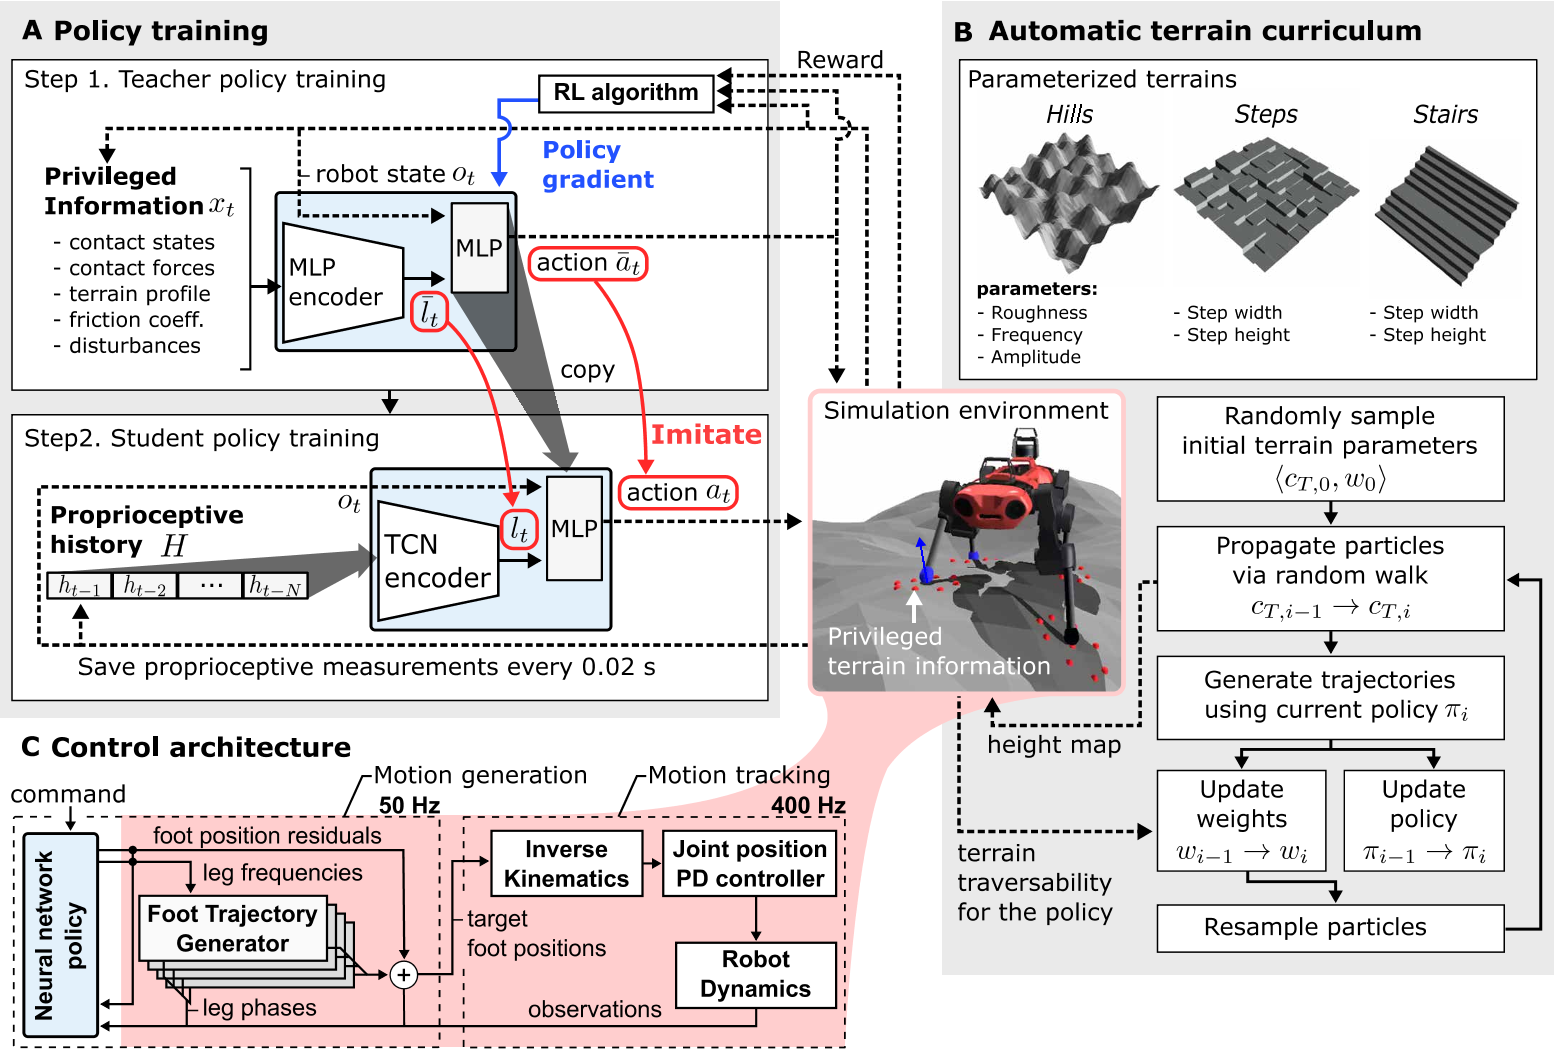
\includegraphics[width=1.0\linewidth]{creating_a_proprioceptive_locomotion_controller.png}
    \caption{Creating a proprioceptive locomotion controller\cite[p7]{Lee_Hwangbo_Wellhausen_Koltun_Hutter_2020}.}
    \label{fig:creating_a_proprioceptive_locomotion_controller}
  \end{figure}

  图\ref{fig:creating_a_proprioceptive_locomotion_controller}是一个只采用本体感知进行机器狗控制的RL策略实现架构。它包括训练定义、地形定义、控制架构。
  \begin{itemize}
    \item 策略训练:整个RL训练采用\emph{特权训练(privileged training)}\cite[p]{Chen_Zhou_Koltun_Krähenbühl_2019}的理念,训练过程分为两个阶段,如图\ref{fig:creating_a_proprioceptive_locomotion_controller}A所示。第一阶段用完善的特权信息作为输入训练出一个\emph{教师策略(teacher policy)};第二阶段仅用本体感知作为输入训练出一个\emph{学生策略(student policy)},学生策略的训练过程通过模仿教师策略实现。实际部署到机器人上的策略是学生策略。
    \item 地形定义:RL训练过程是在一定的地形条件下完成的,如图\ref{fig:creating_a_proprioceptive_locomotion_controller}B所示。对于同样的控制命令,不同的地形条件会产生不同的任务难度。为了能更好地促进训练进步,训练过程中的地形采用\emph{自适应地形课程(adaptive terrain curriculum)},它会从简单地形开始根据训练控制器的性能提升而不断提高地形难度,使得RL控制器时钟面对相对于当前状况的中等地形难度。
    \item 控制架构:整个控制架构采用\emph{调节轨迹生成器(Policies Modulating Trajectory Generators, PMTG)\cite[p]{Iscen_Caluwaerts_Tan_Zhang_Coumans_Sindhwani_Vanhoucke_2018}}架构来提供运动生成的先验。神经网络策略通过合成残差位置命令来调节腿相和运动原语,如图\ref{fig:creating_a_proprioceptive_locomotion_controller}C所示。
  \end{itemize}


\subsection[策略训练]{策略训练}
\subsubsection[教师策略]{教师策略}
整个控制问题被构建成一个\emph{马尔科夫决策过程(Markov Decision Process, MDP)}。MDP是一种用于状态和结果部分随机的离散时间控制过程的数学框架。MDP被定义为一个状态空间$\mathcal{S}$,动作空间$\mathcal{A}$,一个标量奖励函数$\mathcal{R}(s_t,s_{t+1})$,一个转移概率$P(s_{t+1}s_t, a_t)$。一个学习代理从策略$\mathbfit{\pi}(a_t|s_t)$中选择一个动作$a_t$并从环境中获得奖励$r_t$。RL的目的是找到一个优化的策略$\mathbfit{\pi}^*$使得无限时间范围内的折扣奖励总和最大。

状态空间$s_t$定义为:$\langle o_t, x_t\rangle$,其中$o_t$是机器人自身的观测信息,$x_t$是特权信息。
\begin{align}
    s_t\begin{cases}
        o_t\begin{cases}
            proprioceptive\ sensors\\
            state\ estimator\begin{cases}
                base\ velocity\\
                orientation\\
            \end{cases}\\
        \end{cases}\\
        x_t\begin{cases}
            only\ for\ simulation
        \end{cases}\\
    \end{cases}
\end{align}

动作空间$\overline a_t$是一个16维向量,由腿的频率和交的位置残差构成。

奖励函数$\mathcal{R}(s_t|s_{t+1})$定义。

\textcolor{red}{reward function definition details ...}

如图\ref{fig:creating_a_proprioceptive_locomotion_controller}A所示,策略网络由两个MLP模块构成。
第一个MLP模块将$x_t$信息转化成潜在向量$\overline{l}_t$,由于$x_t$中并不含有机器人的状态或指令信息,也就是说他只包含地形信息和接触相关的信息。假设$\overline{l}_t$的作用是驱动自适应行为,比如根据地形轮廓改变脚步间隙大小。然后$\overline{l}_t$和$o_t$再提供给第二个MLP网络来计算动作。

训练采用\emph{信任区域策略优化(Trust Region Policy Optimization, TRPO)}\cite[p]{Schulman_Levine_Moritz_Jordan_Abbeel_2015}。

\subsubsection[学生策略]{学生策略}

学生策略仅能获取$o_t$信息。这里的一个关键假设是潜在特征$\overline{l}_t$可以从本体感觉观察的时间序列$h_t$中恢复(部分),$h_t:=o_t\{f_o, joint\ history, previous\ foot\ position\ targets \}$。

学生策略采用TCN\cite[p]{Bai_Kolter_Koltun_2018}编码器。使用TCN架构的原因是它对输入历史长度提供透明的控制,可以容纳长历史,并且已知对超参数设置具有鲁棒性\cite[p]{Bai_Kolter_Koltun_2018}。

学生策略采用监督学习的方式进行训练,损失函数定义为:
\begin{align}
    \mathcal{L}:=(\overline{a}_t(o_t,x_t)-a_t(o_t,H))^2+(\overline{l}_t(o_t, x_t)-l_t(H))^2
\end{align}
带$(\overline{\cdot})$标识的项是来自教师策略的生成。对于每个访问的状态,教师策略计算其嵌入和动作向量$(\overline{\cdot})$,这些教师策略的输出随即被用作与相应状态相关的监督信号。


\subsection[地形定义]{地形定义}
\textcolor{red}{Adaptive terrain curriculum ...}

\subsection[控制架构]{控制架构}

整个控制架构结构如图\ref{fig:creating_a_proprioceptive_locomotion_controller}C所示。它被分为两大类:\emph{运动生成}、\emph{跟随}。整个系统的输入只有\emph{控制指令}和\emph{本体感知},输出为\emph{关节点位置目标}。

运动生成策略是一种基于周期性腿相位的策略,之前的一些工作中通常利用预定义的脚接触时间表\cite[p7]{Bellicoso_Jenelten_Gehring_Hutter_2018,Barasuol_Buchli_Semini_Frigerio_De_Pieri_Caldwell_2013}。为每条腿都定义一个周期的相位变量$\phi_i\in[0.0,2\pi)$。在每一个时间步长$t$里,$\phi_i = (\phi_{i,0}+(f_0+f_i)t)(\mod 2\pi)$,其中$\phi_{i,0}$是初始相位,$f_0$是一般基础频率,$f_i$是第$i$条腿的频率偏移。我们希望腿在$f_0+f_i\neq 0$时表现出周期性运动,并在接触阶段与地面接触。这里基础频率参考之前开发的传统控制\cite[p7]{Bellicoso_Jenelten_Gehring_Hutter_2018}中鹦鹉步态的值,$f_0=1.25$Hz。

\textcolor{red}{target foot position...}

我们采用PMTG架构来将神经网络集成系统中用来调节控制器的输出。整体实现由四个完全相同的\emph{足迹生成器(foot trajectory generators, FTGs)}和一个\emph{神经网络策略(neural network policy, NNP)}构成。足迹生成器是一个输出每条腿的脚位置的函数:$F(\phi):[0.0,2\pi)\to \mathbb{R}^3$。这个FTG在$f_i$不为零时驱动垂直方向的踱步运动。
\textcolor{gray}{\small
$F(\phi)$的定义如下:
\begin{align}
    F(\phi_i)=\begin{cases}
        (h(-2k^3+3k^2)-0.5)^{H_i}z &k\in[0,1]\\
        (h(2k^3-9k^2+12k-4)-0.5)^{H_i}z &k\in[1,2]\\
        -0.5^{H_i}z & otherwise\\
    \end{cases}
\end{align}
其中$k=2(\phi_i-\pi)/\pi$,$h$是一个表示最大步高的参数。在摆动相位的每一个阶段都是一个连接最高点和最低点的三次Hermite样条曲线,在连接点处曲线具有一阶连续性(一阶导数为零)。其它的周期函数,如$h_i \sin (\phi_i)$可以用于FTG。给定一组合适的$f_0,h,\phi_{i,0}$参数值,机器人就能稳定地在地面上踱步了。比如,文献\cite[p7]{Lee_Hwangbo_Wellhausen_Koltun_Hutter_2020}中使用的值:$f_0=1.25,h=0.2$,$\phi_{i,0}$从$U(0,2\pi)$中采样得到。}
神经网络策略输出$f_{iS}$和脚的目标位置残差($\Delta \mathbfit{r}_{f_i, T}$)。这样,第$i$个脚的目标位置是$\mathbfit{r}_{f_i, T}:=F(\phi_i)+\Delta \mathbfit{r}_{f_i, T}$。

跟随控制是使用解析\emph{逆运动学(inverse kinematics, IK)}和关节点\emph{位置控制(position control)}实现的。在$H_i$中定义的脚位置首先表述在机器人身体系中,然后用IK计算关节点的位置目标。而关节点的位置目标依靠关节点的PD控制器来跟随。使用IK的好处是可以最大化计算效率同时在\emph{仿真到实际(sim-to-real)}的过程中可以复用已有的位置控制驱动器模型\cite[p]{Lee_Hwangbo_Hutter_2019,Hwangbo_Bellicoso_Fankhauser_Huttery_2016}。
